\documentclass{article}
\usepackage[utf8]{inputenc}
\usepackage[italian]{babel}
\usepackage[T1]{fontenc}
\usepackage{float}
\usepackage{graphicx}
\graphicspath{ {./images/}}

\title{Sistemi Operativi}
\author{Ivan A. Arena}
\date{Marzo 2021}

\renewcommand{\contentsname}{Indice}
\renewcommand{\figurename}{Fig.}
\usepackage{xcolor}
\usepackage{listings}
\usepackage{color}
\usepackage{xparse}

\NewDocumentCommand{\codeword}{v}{%
\texttt{\textcolor{blue}{#1}}%
}


\definecolor{mygreen}{rgb}{0,0.6,0}
\definecolor{mygray}{rgb}{0.5,0.5,0.5}
\definecolor{mymauve}{rgb}{0.58,0,0.82}

\lstset{ 
  backgroundcolor=\color{white},   % choose the background color; you must add \usepackage{color} or \usepackage{xcolor}; should come as last argument
  basicstyle=\footnotesize,        % the size of the fonts that are used for the code
  breakatwhitespace=false,         % sets if automatic breaks should only happen at whitespace
  breaklines=true,                 % sets automatic line breaking
  captionpos=b,                    % sets the caption-position to bottom
  commentstyle=\color{mygreen},    % comment style
  deletekeywords={...},            % if you want to delete keywords from the given language
  escapeinside={\%*}{*)},          % if you want to add LaTeX within your code
  extendedchars=true,              % lets you use non-ASCII characters; for 8-bits encodings only, does not work with UTF-8
  firstnumber=1000,                % start line enumeration with line 1000
  frame=none,	                   % adds a frame around the code
  keepspaces=true,                 % keeps spaces in text, useful for keeping indentation of code (possibly needs columns=flexible)
  keywordstyle=\color{blue},       % keyword style
  language=Octave,                 % the language of the code
  morekeywords={*,...},            % if you want to add more keywords to the set
  numbers=none,                    % where to put the line-numbers; possible values are (none, left, right)
  numbersep=5pt,                   % how far the line-numbers are from the code
  numberstyle=\tiny\color{mygray}, % the style that is used for the line-numbers
  rulecolor=\color{black},         % if not set, the frame-color may be changed on line-breaks within not-black text (e.g. comments (green here))
  showspaces=false,                % show spaces everywhere adding particular underscores; it overrides 'showstringspaces'
  showstringspaces=false,          % underline spaces within strings only
  showtabs=false,                  % show tabs within strings adding particular underscores
  stepnumber=2,                    % the step between two line-numbers. If it's 1, each line will be numbered
  stringstyle=\color{mymauve},     % string literal style
  tabsize=2,	                   % sets default tabsize to 2 spaces
  title=\lstname                   % show the filename of files included with \lstinputlisting; also try caption instead of title
}

\begin{document}

\maketitle

\noindent Testo di appunti del corso di \textit{Sistemi Operativi} della Facoltà di Informatica dell'Università degli Studi di Padova.

\tableofcontents

\section{Introduzione} Un \textbf{sistema operativo} (\textbf{S/O}) è un insieme di utilità progettate per gestire le risorse fisiche e logiche di un elaboratore fornendo all'utente un'astrazione più semplice e potente, costituita da una \textbf{macchina virtuale}, un ambiente in cui la memoria è virtualizzata ed è possibile eseguire applicazioni senza particolari conoscenze. 

\section{Programmi e processi} Si dice \textbf{programma} un codice che esegue una o più istruzioni; un programma in esecuzione è detto, invece, \textbf{processo}. In un sistema operativo i processi (\textit{utente} e \textit{di sistema}) avanzano \textbf{concorrentemente} (non simultaneamente) secondo diverse politiche di ordinamento, garanti della \textit{fairness}, decise nello \textbf{scheduling}.

\subsection{Risorse} Una \textbf{risorsa} è un qualsiasi elemento fisico o logico necessario alla creazione, esecuzione ed avanzamento di processi e può essere: \begin{itemize}
    \item Durevole o consumabile;
    \item Ad accesso atomico o divisibile;
    \item Ad accesso individuale o molteplice;
\end{itemize} 
Le risorse del tipo I/O sono gestite da un programma specifico, il \textbf{BIOS}.

\subsection{Stati di avanzamento dei processi} 

\begin{figure}[H]
    \centering
    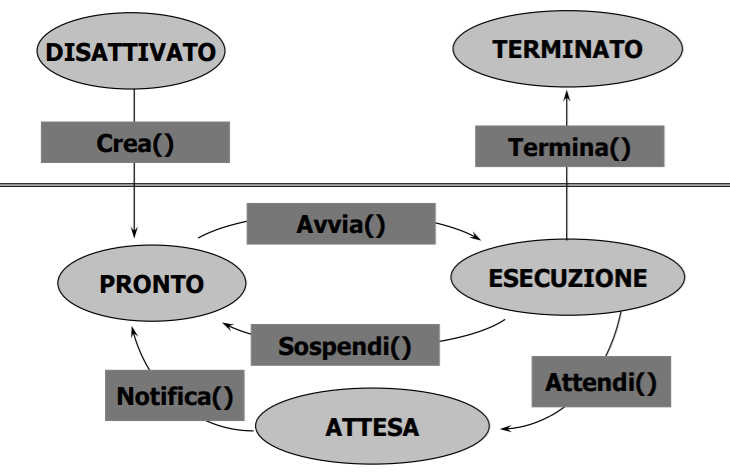
\includegraphics[scale=0.5]{statoprocesso}
    \caption{Stati di avanzamento dei processi.}
    \label{fig:stato_processi}
\end{figure}

\noindent Come illustrato in Fig.  \ref{fig:stato_processi}, un processo \textbf{disattivato} viene caricato in memoria tramite una chiamata di sistema che crea una struttura dati detta \textbf{Process Control Block} (\textbf{PCB}), entra in stato di \textbf{pronto}, va in \textbf{esecuzione} in base alla priorità attribuitagli, dove può \textbf{terminare}, essere \textbf{prerilasciato} (o \textbf{sospeso}) per dare spazio ad un altro processo, o messo in \textbf{attesa}.

\subsection{Gestione dei processi} La gestione dei processi è affidata al nucleo del sistema operativo, il \textbf{kernel}. Il componente che gestisce gli scambi tra i processi in esecuzione è il \textbf{dispatcher}. I processi in stato di pronto sono accodati in una struttura detta \textbf{lista dei pronti} (\textbf{ready list}), spesso del tipo \textbf{First-Come-First-Served} (\textbf{FCFS}). I processi possono essere \textbf{CPU-bound}, attività dalla durata molto lunga, o \textbf{I/O-bound}, comprendenti attività di breve durata sulla CPU ed altre di I/O molto lunghe. Quest'ultimi sono penalizzati dalla tecnica FCFS, motivo per cui vengono messi a disposizione di ogni processo uguali \textbf{quanti} di tempo (\textbf{round-robin}) e vengono istituite code diverse in base alla priorità o alla categoria dei vari processi.

\section{Sincronizzazione dei processi} Spesso, i processi condividono risorse e servono meccanismi di \textbf{sincronizzazione di accesso} per gestirne la condivisione.

\paragraph{Esempio:} Siano $A$ e $B$ due processi che condividono la variabile $x = 10$; $A$ incrementa $x$ di $2$, $B$ decrementa $x$ di $4$. $A$ e $B$ leggono $x$ uno dopo l'altro, leggendo, quindi, entrambi $10$. Allora $A$ scriverà $12$, mentre $B$ scriverà $6$. Il risultato desiderato era invece $8 (10+2-4)$.

\subsection{Race condition e regione critica} Quando, come nel caso di cui sopra, il risultato finale dell'esecuzione di processi dipende dalla temporizzazione o dalla sequenza con cui vengono eseguite le loro istruzioni si verifica una \textbf{race condition}, in una regione di codice detta \textbf{regione} (o \textbf{sezione}) \textbf{critica}. Una soluzione al problema della sincronizzazione dei processi è ammissibile se soddisfa le seguenti quattro condizioni:
\begin{itemize}
    \item Garantire accesso esclusivo (\textbf{mutua esclusione});
    \item Garantire attesa finita;
    \item Non fare assunzioni sull'ambiente di esecuzione;
    \item Non subire condizionamenti dai processi esterni alla sezione critica.
\end{itemize}

\paragraph{} Un altro problema tipico è quello dello stallo (come vedremo nella sottosezione successiva) bloccante (\textbf{deadlock}) o non-bloccante (\textbf{starvation}). Le condizioni necessarie e sufficienti affinché si verifichi uno stallo sono:

\begin{itemize}
    \item Accesso esclusivo ad una risorsa condivisa;
    \item Accumulo di risorse;
    \item Inibizione di prerilascio;
    \item Condizione di attesa circolare.
\end{itemize}

\paragraph{N.B.:} \textit{Necessarie} e \textit{sufficienti} significa che basta impedire il verificarsi di anche una sola di queste per impedire lo stallo.

\paragraph{} Per affrontare uno stallo possiamo optare, principalmente, per tre strategie: prevenzione (a tempo di esecuzione o prima), riconoscimento e recupero, \textbf{indifferenza} (quella più semplice ed efficace).

\subsection{Problema produttore-consumatore} Il problema del \textbf{produttore-consumatore} nasce in due casi principali: \begin{itemize}
    \item Inizia il \textit{consumatore}, legge \codeword{count == 0} ma viene prerilasciato prima di eseguire l'istruzione \codeword{sleep()}; a quel punto, viene eseguito il \textit{produttore}, che incrementa \codeword{count} (portandolo ad \codeword{1}) ma non sveglia il \textit{consumatore}, poiché non addormentato, allora, quando il produttore verrà prerilasciato, il \textit{consumatore} si addormenterà e la condizione \codeword{count == 1} non sarà mai vera, poiché il \textit{produttore} continuerà ad incrementare \codeword{count} fino a \codeword{count == N}, quando si addormenterà, causando un deadlock;
    \item Analogamente, inizia il \textit{produttore} e produce fino a \codeword{count == N} ma viene prerilasciato prima di eseguire l'istruzione \codeword{sleep()}; allora, il \textit{consumatore} decrementerà \codeword{count} fino ad \codeword{N-1} e non sveglierà il \textit{produttore}, poiché non addormentato, e consumerà tutti gli elementi del buffer per poi addormentarsi, causando un deadlock.
\end{itemize}

\begin{figure}[H]
    \centering
    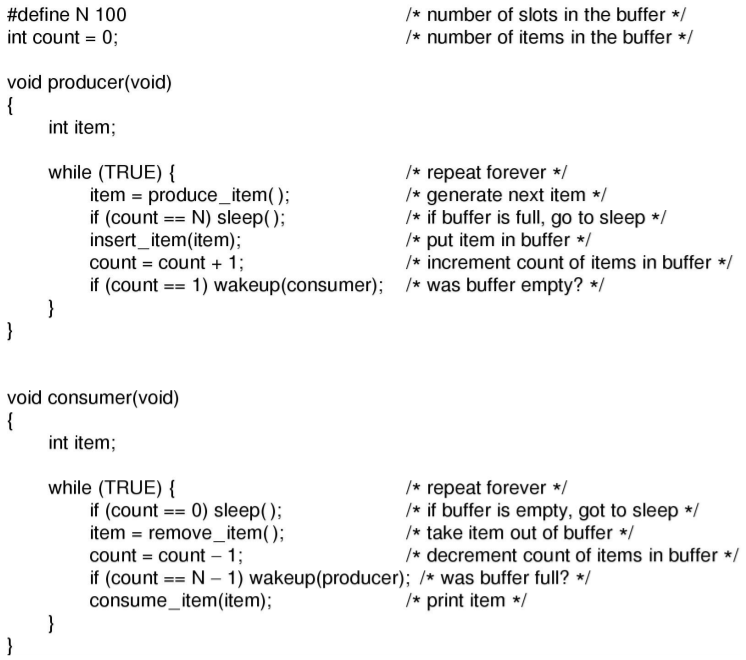
\includegraphics[scale=0.5]{produttoreconsumatore.png}
    \caption{Problema produttore-consumatore.}
    \label{fig:prod-cons}
\end{figure}

\subsection{Semafori} Una possibile soluzione a problemi come quello del produttore-consumatore coinvolge l'uso di una variabile atomica detta \textbf{semaforo}, \textbf{binario} (assume solo valori booleani) o \textbf{contatore} (consente più accessi condivisi).

\begin{figure}[H]
    \centering
    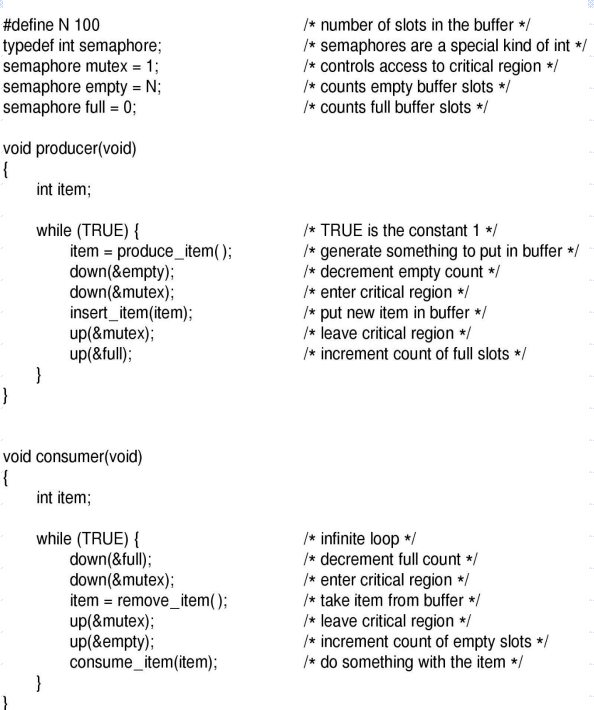
\includegraphics[scale=0.5]{solproduttoreconsumatore.png}
    \caption{Soluzione al problema produttore-consumatore mediante l'uso dei semafori.}
    \label{fig:sol-prod-cons-sem}
\end{figure}

\subsection{Monitor} L'uso dei semafori da utente è, però, rischioso, perciò viene affidato ad una struttura di variabili e sottoprogrammi detta \textbf{monitor}, che definisce la regione critica e agisce da compilatore. Solo i suoi sottoprogrammi possono modificare le variabili interne ad un monitor. Tali strutture, oltre a garantire la mutua esclusione, impiegano due procedure, \codeword{wait} e \codeword{signal}, rispettivamente per forzare l'attesa del chiamante ed il risveglio del processo in attesa. Inoltre, non sono utilizzabili per lo scambio di informazioni tra elaboratori.

\subsection{Message Passing} Un'altra possibilità per sincronizzare i processi è offerta dal \textbf{message passing} (\textbf{scambio messaggi}), che permette, al contrario dei monitor, la sincronizzazione tra dispositivi distinti ed impiega le funzioni base \codeword{send(destination, &msg)} e \codeword{receive(source, &msg)}.

\begin{figure}[H]
    \centering
    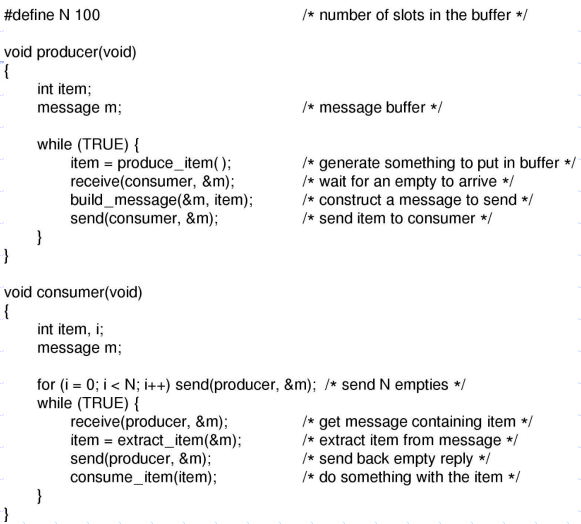
\includegraphics[scale=0.5]{solproduttoreconsumatore2.png}
    \caption{Soluzione al problema produttore-consumatore mediante lo scambio messaggi}
    \label{fig:sol-prod-cons-mes}
\end{figure}

\subsection{Barriere} Le \textbf{barriere} sono uno strumento che permette di sincronizzare gruppi di processi bloccandoli finché non la raggiungono tutti.

\subsection{Problema dei filosofi} Ad un tavolo circolare sono seduti 5 filosofi, che alternano momenti in cui pensano a momenti in cui mangiano. Per mangiare, ogni filosofo necessita di due posate, quella alla sua destra e quella alla sua sinistra. Se tutti i filosofi cominciano a mangiare prendendo la prima posata ogni filosofo rimarrà senza la seconda, in attesa circolare, causando un deadlock.

\begin{lstlisting}[language=java]
// Soluzione al problema dei filosofi mediante l'uso di semafori.
int semaforo f[i] = 1;

// Per evitare il deadlock inseriamo un filosofo mancino, che prende prima la posata sinistra e poi quella destra
Filosofo(i) {
    while(1) {
        <pensa>
        if(i == X) { // Filosofo mancino X
            P(f[(i+1) % N]);
            P(f[i]);
        } else {
            P(f[i]);
            P(f[(i+1) % N]);
        }
        <mangia>
        V(f[i]);
        V(f[(i+1) % N]);
    }
}
\end{lstlisting}

\begin{figure}[H]
    \centering
    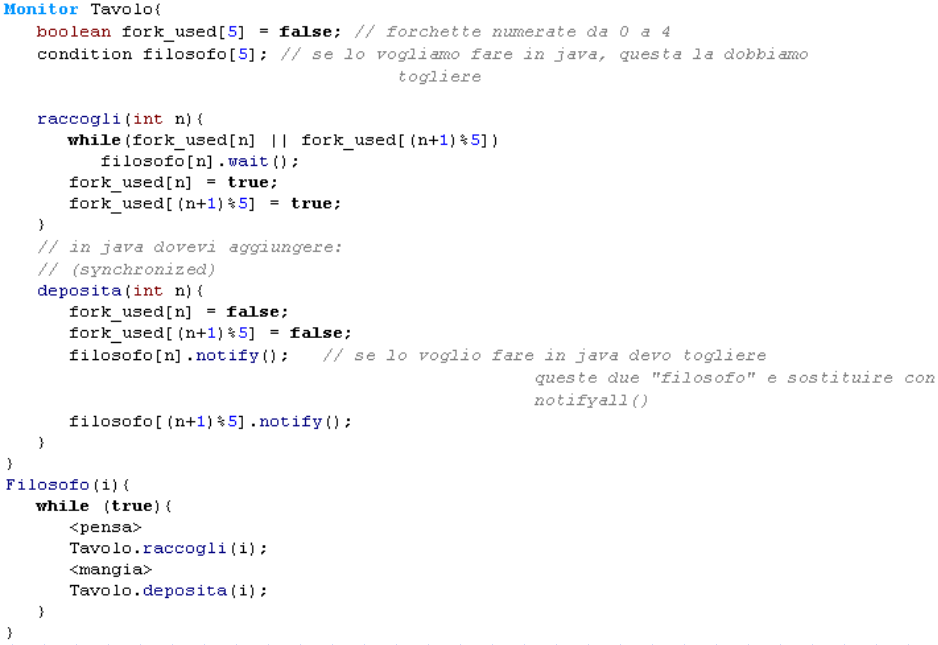
\includegraphics[scale=0.5]{filosofi-monitor.png}
    \caption{Soluzione al problema dei filosofi mediante l'uso di monitor.}
    \label{fig:filo-monitor}
\end{figure}

\subsection{Problema dei lettori e degli scrittori} Un grande database deve essere letto e scritto. Più lettori possono accedervi contemporaneamente mentre gli scrittori possono solo quando non ci sono lettori.

\begin{figure}[H]
    \centering
    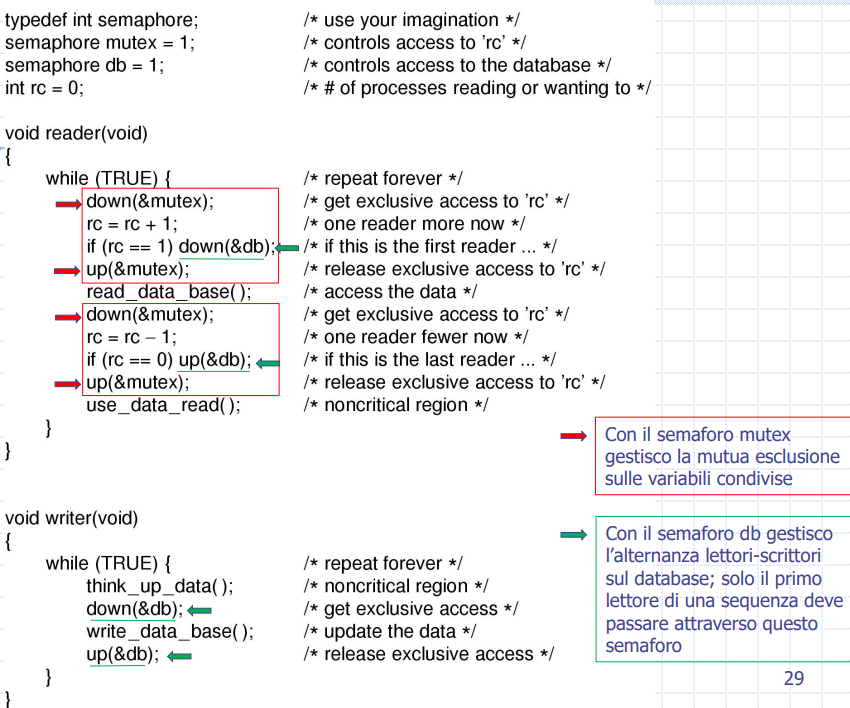
\includegraphics[scale=0.5]{lettorescrittore.png}
    \caption{Soluzione al problema dei lettori e degli scrittori mediante l'uso di semafori.}
    \label{fig:filo-monitor}
\end{figure}

\subsection{Problema del barbiere sonnolento} Un barbiere dorme sulla poltrona se non ci sono clienti. Il primo cliente sveglia il barbiere e quelli successivi si siedono, su un numero limitato di sedie, in attesa che il barbiere finisca.

\begin{figure}[H]
    \centering
    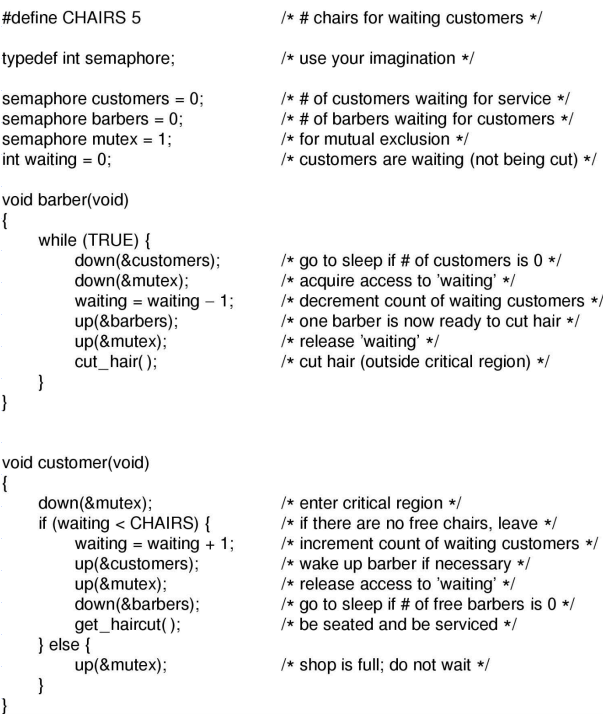
\includegraphics[scale=0.5]{barb.png}
    \caption{Soluzione al problema del barbiere sonnolento mediante l'uso di semafori.}
    \label{fig:barb}
\end{figure}

\section{Ordinamento dei processi} Le informazioni sulla priorità di un certo processo sono contenute nel suo PCB (Process Control Block). Nella coda dei pronti troviamo solitamente un puntatore al PCB di ogni processo in coda. Una decisione di scheduling è necessaria alla creazione di un processo, alla terminazione, al blocco o all'interruzione I/O. I processi possono essere alternati con \textbf{scambio a prerilascio} (necessita di clock), tramite un meccanismo esterno, o con \textbf{scambio cooperativo} (il processo decide da solo).

\subsection{Politiche e meccanismi} I \textbf{meccanismi} sono le sezioni del S/O che mettono in pratica le scelte di ordinamento e di gestione dei processi e risiedono nel nucleo; le \textbf{politiche} sono, invece, determinate fuori dal nucleo, nello spazio applicazioni.

\subsection{Classificazione di sistemi} I sistemi operativi si dividono in tre classi generali: 
\begin{itemize}
    \item \textbf{Sistemi a lotti} (\textit{batch}): ordinamento predeterminato e lavori poco urgenti e di lunga durata; prerilascio non necessario; \textbf{obiettivi delle politiche:} massima rapidità per singolo lavoro (\textit{\textbf{turn-around}});
    \item \textbf{Sistemi interattivi}: grande varietà di attività, prerilascio essenziale; \textbf{obiettivi delle politiche:} tempo di risposta (rispetto alla percezione dell'utente);
    \item \textbf{Sistemi a tempo reale}: lavori brevi ma urgenti, prerilascio possibile; \textbf{obiettivi delle politiche:} rispetto delle scadenze temporali (\textit{\textbf{deadline}}) e predicibilità.
\end{itemize}

Le politiche di ordinamento dovrebbero rispettare tre cose: \textbf{equità} (\textit{fairness}), \textbf{coerenza} (\textit{enforcement}) e \textbf{bilanciamento}.

\subsection{Politiche di ordinamento} \paragraph{Importante:} Lo \textbf{scheduler} fissa la politica di ordinamento, il \textbf{dispatcher} ne attua le scelte.

\begin{itemize}
    \item \textbf{Tempo di risposta} = Tempo trascorso dall'entrata in coda fino all'inizio della prima esecuzione;
    \item \textbf{Tempo di attesa} = Tempo passato in coda;
    \item \textbf{Tempo di esecuzione} = Durata effettiva del lavoro (senza contare le attese).
    \item \textbf{Tempo di turn-around} = Tempo di attesa + Tempo di esecuzione;
\end{itemize}


\subsubsection{Sistemi a lotti} \begin{itemize}
    \item \textbf{FCFS} (\textbf{First Come First Served}): senza prerilascio né priorità, basso utilizzo delle risorse;
    \item \textbf{SJF}: senza prerilascio, richiede conoscenze dei tempi di esecuzione richiesti, non è equo con lavori non presenti dall'inizio;
    \item \textbf{SRTN} (\textbf{Shortest Remaining Time Next}): variante di SJF con prerilascio, tiene conto dei nuovi processi quando arrivano ed esegue quello più veloce a completare.
\end{itemize}

\paragraph{N.B.:} In genere, si parla di \textbf{lavori} quando operiamo senza prerilascio e di \textbf{processi} quando operiamo con prerilascio.

\subsubsection{Sistemi interattivi} \begin{itemize}
    \item \textbf{OQ} (\textbf{Ordinamento a Quanti}, es.: Round Robin (RR)): con prerilascio ma senza priorità;
    \item \textbf{OQP} (\textbf{Ordinamento a Quanti con Priorità}): con prerilascio e priorità, quanti diversi per livello di priorità;
    \item \textbf{GP} (\textbf{con Garanzia per Processo}): con prerilascio e con promessa una data quantità di tempo di esecuzione ($1/n-processi$), esegue prima il lavoro maggiormente penalizzato rispetto alla promessa;
    \item \textbf{SG} (\textbf{Senza Garanzia}): con prerilascio e priorità a, ogni processo riceve più o meno numeri, segue un'estrazione periodica (più numeri = più probabilità di vittoria);
    \item \textbf{GU} (\textbf{con Garanzia per Utente}): Come GP ma con garanzia riferita a ciascun utente ($1/n-utenti$).
\end{itemize}

\subsubsection{Sistemi in tempo reale} \begin{itemize}
    \item \textbf{Modello semplice} (\textbf{\textit{cyclic executive}}): processi periodici con caratteristiche note, un ciclo maggiore (\textit{major cycle}) è suddiviso in N cicli minori (\textit{minor cycles}) di durata fissa che racchiudono sottosequenze di processi;
    \item \textbf{Ordinamento a priorità fissa}: preferibilmente con prerilascio a priorità assegnata secondo il periodo (priorità maggiore per periodo più breve); % RISCHIO INVERSIONE DI PRIORITà
    \item \textbf{Calcolo del tempo di risposta};
\end{itemize}

\section{Gestione della memoria} La componente del S/O che si occupa di soddisfare le esigenze di memoria dei processi è il \textbf{gestore della memoria}. Per i sistemi \textbf{monoprogrammati} (quelli che eseguono un solo processo alla volta) l'unica scelta progettuale rilevante è decidere dove allocare la memoria del S/O.

\subsection{Frammentazione} La \textbf{frammentazione} è lo spreco di memoria e può essere \textbf{interna}, quando la memoria è divisa in blocchi di uguali dimensioni ed alcuni vengono riempiti solo in parte, o \textbf{esterna}, quando la memoria è divisa, invece, in blocchi di dimensione variabile e rimangono delle aree di memoria non copribili da blocchi.

\subsection{Rilocazione e protezione} La \textbf{rilocazione} è l'interpretazione degli indirizzi emessi da un processo in relazione alla sua collocazione corrente in memoria; la \textbf{protezione} assicura che ogni processo operi soltanto nello spazio di memoria ad esso permissibile.

\subsection{Swapping} Lo \textbf{swapping} è una tecnica per alternare processi in memoria principale senza garantire allocazione fissa, assegnando, infatti, partizioni diverse nel tempo, assegnate ad hoc. Può provocare frammentazione esterna ed occorre ricompattare periodicamente la memoria sprecando non poco tempo.

\subsection{Strutture di gestione} È essenziale tenere traccia dello stato d'uso della memoria, e lo si fa o per mezzo di \textbf{mappe di bit}, o per mezzo di \textbf{liste collegate}, in cui ogni elemento è un segmento e l'allocazione avviene secondo strategie di:
\begin{itemize}
    \item \textbf{First fit}: il primo segmento libero ampio abbastanza; 
    \item \textbf{Next fit}: come \textit{first fit} ma cercando solo in avanti;
    \item \textbf{Best fit}: il segmento libero più adatto;
    \item \textbf{Worst fit}: il segmento libero più ampio;
    \item \textbf{Quick fit}: liste diverse per ampiezze tipiche.
\end{itemize}

\subsection{Memoria virtuale} La memoria virtuale nasce per ovviare alle crescenti esigenze di spazio dei singoli processi permettendo di allocare in RAM processi maggiori della stessa, caricandone solo la parte strettamente necessaria e mettendo il resto su disco (come \textbf{overlay} (divisione di un processo in parti) ma senza intervento del programmatore). La memoria virtuale è gestita tramite \textbf{paginazione} o tramite \textbf{segmentazione}. Gli indirizzi virtuali generati dal processo vengono trasformati in fisici dalla \textbf{MMU}.

\subsection{Paginazione} La memoria virtuale è suddivisa in unità a dimensione fissa dette \textbf{pagine}; la RAM è suddivisa in \textbf{cornici} (\textbf{page frames}), ampie quanto le pagine. I trasferimenti da e verso disco avvengono sempre in  pagine intere. Per sapere se una pagina è in RAM le si assegna un \textbf{bit di presenza}. Se viene riferita una pagina assente si genera un \textbf{page fault}. 

\subsubsection{Strutture} Ogni processo ha una sua \textbf{tabella delle pagine}, contenente per ogni pagina virtuale la corrispondente locazione fisica.
La RAM viene scansionata dal \textbf{TLB} (\textbf{Translation Lookaside Buffer}), realizzata in software o in hardware nell'MMU, per verificare la presenza o meno di una pagina. Data la grandezza delle tabelle delle pagine nelle architetture moderne viene adottata la soluzione della \textbf{tabella invertita}, consiste nell'indirizzare in ogni riga un page frame invece edi una pagina (implicando una traduzione più complessa), realizzata come una \textbf{tabella hash} (\textbf{hash table}).

\subsubsection{Rimpiazzo} Quando si produce un \textit{page fault} il S/O deve rimpiazzare una pagina (salvando su disco la pagina rimossa se è stata modificata (\textit{nda} come quando si lavora con la cache)). Il \textbf{rimpiazzo ottimale} (\textbf{optimal replacement}) rimpiazza la pagina che non sarà usata per maggior tempo, ma non è realizzabile in quanto il S/O non può prevedere a quali pagine il progesso accederà in futuro. Le sue approssimazioni sono:
\begin{itemize}
\item \textbf{NRU} (\textbf{Not Recently Used}): ad ogni page frame vengono assegnati un \textbf{bit M} (\textbf{modified}) ed un \textbf{bit R} (\textbf{referenced}) come contatori e viene rimpiazzata una pagina casuale nella classe non vuota ad indice più basso tra classe 0 (non riferita, non modificata), 1 (non riferita, modificata), 2 (riferita, non modificata) e 3 (riferita, modificata);
\item \textbf{FIFO}: rimpiazza la pagina entrata meno recentemente in RAM;
\item \textbf{Second chance}: corregge FIFO rimpiazzando solo le pagine con bit R uguale a $0$ (può degenerare in FIFO);
\item \textbf{Orologio}: come SC ma i page frame sono mantenuti in una lista circolare;
\item \textbf{LRU} (\textbf{Least Recently Used}): approssima l'algoritmo ottimale ma necessita di un hardware dedicato e della lista aggiornata ogni volta che si fa un riferimento;
\item \textbf{NFU} (\textbf{Not Frequently Used}): Realizzabile a software, aggiorna periodicamente un contatore per ogni page frame ma non dimentica nulla;
\item \textbf{Aging}: come NFU ma valuta solo periodicamente;
\item \textbf{WS approssimato} (vedi sotto): simile all'aging;
\item \textbf{WS approssimato con orologio} (vedi sotto): come WS approssimato ma con i page frame dipsosti in una lista circolare.
\end{itemize}

\paragraph{WS:} Il \textbf{Working Set} (\textbf{WS}) è l'insieme delle pagine che un processo ha in uso ad un dato istante. Se esso viene caricato prima dell'esecuzione si ha \textbf{prepaging} e si evita il page fault, mentre se la memoria non è sufficiente a contenerlo si ha il fenomeno di \textbf{thrashing} (rimpiazzi indesiderati).

\paragraph{N.B.: Aumentare il numero delle page frame non implica necessariamente una diminuzione dei page fault (\textbf{anomalia di Belady})}.

\subsection{Segmentazione} La memoria può anche essere divisa in \textbf{segmenti} o in \textbf{segmenti paginati}. Per accedervi, un programma carica il \textbf{selettore} del segmento, che punta ad un \textbf{descrittore} contenente una base di indirizzo alla quale bisogna sommare un offset per trovare l'indirizzo fisico (o logico nel caso di segmentazione paginata) cercato.

\section{File System} Il File System è il serivizio di S/O progettato per realizzare, conservare, mantenere dati di diverso tipo e dimensione e fornirne l'accesso alle diverse applicazioni. Il \textbf{file} è un insieme di dati trattati unitariamente e strutturati in tre livelli:

\begin{itemize}
    \item Livello \textbf{utente}: l'applicativo associa autonomamente significato al contenuto del file;
    \item Livello di \textbf{struttura logica}: il S/O organizza i dati in strutture logiche per facilitarne il trattamento;
    \item Livello di \textbf{struttura fisica}: il S/O mappa le strutture logiche su quelle fisiche della memoria secondaria disponibile.
\end{itemize}

\subsection{Struttura logica di file} Le possibili strutture logiche di un file sono a \textbf{sequenza} di byte (puntatore all'inizio del file), a \textbf{record} di lunghezza e struttura interna fissa (il S/O deve conoscerne la struttura, obsoleto) o variabile (una tabella contiene i puntatori alle chiavi / \textit{\textbf{keys}} che descrivono ogni record).

\subsubsection{Modalità di accesso} \begin{itemize}
    \item \textbf{Accesso sequenziale:} un puntatore indirizza il record corrente ed avanza ad ogni lettura o scrittura: si può scrivere solo sulla coda e leggere sequenzialmente (se il file da leggere è stato oltrepassato è necessario tornare al primo indirizzo e ricominciare la ricerca);
    \item \textbf{Accesso diretto:} i record sono posti in posizione arbitraria, determinata rispetto dalla base;
    \item \textbf{Accesso indicizzato:} per ogni file una tabella contenente gli \textbf{offset} dei rispettivi record; consente anche accesso sequenziale.
\end{itemize}

\subsubsection{Classificazione di file}
\begin{itemize}
    \item \textbf{File regolari:} contenuto ASCII o binario su cui l'utente può operare normalmente;
    \item \textbf{File catalogo (directory):} descrivono l'organizzazione di gruppi di file (file e directory risiedono in aree logiche distinte);
    \item \textbf{File speciali:} rappresentano logicamente dispositivi orientati a carattere o a blocco (\textit{solo UNIX / GNU / LINUX}).
\end{itemize}

\subsection{Struttura di directory} A livello utente, una struttura di directory deve essere efficiente (realizzare e trovare un file deve essere semplice e veloce) e fornire libertà di denominazione e raggruppamento (logico). Rispetto all'organizzazione, le directory possono essere:

\begin{itemize}
    \item \textbf{A livello singolo:} tutti i file sono elencati su una lista lineare, ciascuno con il proprio nome (gestione onerosa all'aumentare dei file);
    \item \textbf{A due livelli:} una \textbf{root directory} contiene una \textbf{User File Directory} (\textbf{UFD}) per ciascun utente di sistema, il quale può vedere solo la propria UFD; i file sono localizzati tramite \textbf{percorso} (\textbf{path}) e i programmi di sistema possono essere copiati su tutte le UFD o (meglio) posti in una directory di sistema condivisa;
    \item \textbf{Ad albero}: Numero arbitrario di livelli sottostanti alla root directory;
    \item \textbf{A grafo (aciclico o generalizzato):}  un file può appartenere contemporaneamente a più directory; UNIX e GNU/Linux utilizzano \textbf{link} tra il nome reale del file e la sua presenza virtuale, \textbf{hard link} quando un puntatore diretto ad un file viene inserito in un'altra directory remota dello stesso file system (due vie d'accesso dirette), o \textbf{symbolic (soft) link}, quando, invece, viene creato un file speciale contenente il cammino del file originario di qualunque FS (una sola via d'accesso);
\end{itemize}

\subsection{Realizzazione del file system} I file system sono memorizzati su dischi il cui settore 0 contiene le informazioni di inizializzazione del sistema (\textbf{Master Boot Record}), eseguita dal BIOS.

\subsubsection{Realizzazione di file} A livello fisico un file è un insieme di blocchi di disco, allocati in tre modi possibili:

\begin{itemize}
    \item \textbf{Allocazione contigua:} la memorizzazione avviene su blocchi \textbf{consecutivi}, ogni file è descritto dall'indirizzo del suo primo blocco ed il numero di blocchi utilizzati; ogni modifica di file comporta il rischio di frammentazione esterna;
    \item \textbf{Allocazione a lista concatenata:} il file è identificato dal puntatore al suo primo blocco, che è anche il puntatore ad una lista concatenata di blocchi, contenenti ognuna parte del file (un solo blocco guasto corrompe l'intero file);
    \item \textbf{Allocazione a lista indicizzata:} i blocchi contengono solo dati e i puntatori si trovano in strutture apposite, di forma tabulare (\textbf{FAT}, \textbf{File Allocation Table}) o indicizzata (\textbf{i-node}, nodo indice), consentendo accesso sequenziale e diretto senza causare frammentazione esterna. 
    
\paragraph{FAT:}tabella ordinata di puntatori a blocchi (\textbf{cluster}); un file è una catena di indici e la FAT relativa ai file in uso deve risiedere interamente in RAM; la sua dimensione non dipende dalla grandezza dei file al suo interno bensì dalla dimensione della partizione di disco e dall'ampiezza dei suoi indirizzi;

\paragraph{i-node:}una struttura indice ad ampiezza limitata contenente gli attributi di ogni file ed i puntatori ai suoi blocchi, quindi non è influenzata dalla contiguità (o meno) dei blocchi; in RAM una tabella per i soli file in uso. Per file medi e grandi (troppi puntatori per un singolo i-node) gli i-node possono puntare rispettivamente uno o più blocchi i-node intermedi;

\end{itemize}

\subsubsection{Gestione dei blocchi liberi} Si può optare per una lista concatenata dei blocchi liberi (come in FAT) o per un vettore di bit (\textbf{bitmap}), dove ogni bit indica lo stato del corrispondente blocco (0 libero, 1 occupato).

\subsection{Integrità del File System} I blocchi danneggiati vengono gestiti \textbf{via software}, occupandoli con un falso file, o \textbf{via hardware}, creando e mantenendo in un settore del disco un elenco di blocchi danneggiati e dei loro sostituti. Il FS viene salvato su nastro (tempi lunghi) o su disco, con partizione di \textbf{back-up} o mediante \textbf{RAID}. Ogni blocco può appartenere ad una delle due liste dei blocchi in uso e liberi, se appartiene a due si ha una duplicazione, se a nessuna si ha una perdita. Una parte della memoria principale viene usata come cache per alcuni blocchi e le modifiche vengono ricopiate immediatamente su disco (\textbf{write-through}, MS-DOS) o con un refresh periodico (\textbf{sync}, UNIX / GNU / Linux).

\end{document}
